\chapter{Project Management}

This chapter details the project management approach used throughout this 13-week research project. It describes the planning, execution, and monitoring strategies that facilitated the successful completion of the research objectives within the allocated timeframe. The chapter covers the project schedule, risk management strategies, quality assurance processes, and considerations of social, legal, ethical, and professional aspects.

The 13-week project was organised into sequential phases with specific milestones to ensure systematic progression and timely completion. Figure \ref{fig:gantt_chart} presents the Gantt chart that illustrates the project timeline and phase dependencies.

\begin{figure}[ht]
    \centering
    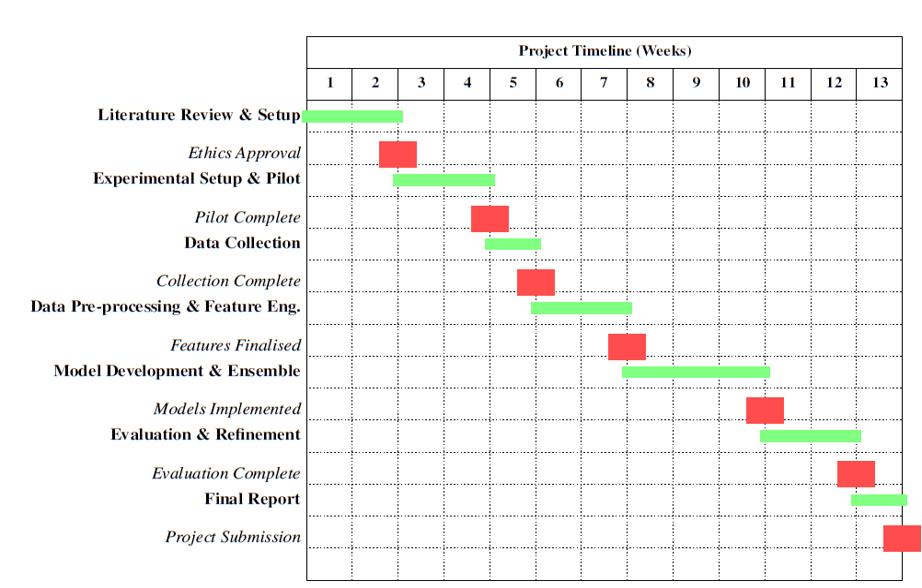
\includegraphics[width=\textwidth]{images/gantt_chart.png}
    \caption{Gantt chart depicting the 13-week project schedule and milestones}
    \label{fig:gantt_chart}
\end{figure}

\section{Project Schedule and Execution}

\subsection{Project Phases}

The project was divided into the following key phases, each with defined deliverables and timeframes:

\begin{enumerate}
    \item \textbf{Project Initiation (Week 1):} This phase involved refining the research question, establishing project objectives, and developing the initial project plan. Key activities included a preliminary review of the literature to establish the current state of research in malware detection for IoT environments.
    
    \item \textbf{Dataset Acquisition and Exploration of the data set (Weeks 2-3):} This phase focused on acquiring the CTU-IoT Malware dataset, performing an initial exploratory data analysis, and developing a complete understanding of the characteristics of the data. Statistical analysis was conducted to identify key features and distribution patterns.
    
    \item \textbf{Data Preprocessing and Feature Engineering (Weeks 3-5):} During this critical phase, data cleaning techniques were applied to address missing values and outliers. Feature engineering strategies were developed based on domain knowledge and exploratory findings, resulting in a set of derived features to enhance model performance.
    
    \item \textbf{Model Development and Initial Testing (Weeks 5-7):} This phase involved implementing and training multiple machine learning models, including Random Forest, SVM, and XGBoost. The initial performance evaluation was performed using cross-validation techniques.
    
    \item \textbf{Hyperparameter Optimisation (Weeks 7-8):} Systematic hyperparameter tuning was performed using RandomizedSearchCV to optimise the model performance. This iterative process required substantial computational resources and careful evaluation of the results.
    
    \item \textbf{Comprehensive Evaluation (Weeks 8-10):} The final performance of the model was rigorously assessed using the held-out test set. Detailed analysis of the results was performed during this phase, including confusion matrices, importance of characteristics, and performance metrics.
    
    \item \textbf{Documentation and Dissertation Writing (Weeks 10-13):} The final phase focused on documenting the research methodology, findings, and implications. This included preparing visualisations, tables, and formal documentation of the complete research process, culminating in the final dissertation.
\end{enumerate}


\section{Risk Management}

Risk management was a critical component of the project, given the complexity and potential challenges associated with machine learning research in cybersecurity. The following sections outline the key risks identified, their potential impact, and the strategies employed to mitigate them.

Several key risk mitigation strategies were employed during the project. To address dataset limitations, a thorough exploratory data analysis was performed early to understand its characteristics and constraints. Although the predominance of scanning attacks was identified, the dataset was deemed sufficiently valuable for the research objectives. The scope of the research and the interpretation of the results were carefully adjusted to acknowledge these limitations. Alternative datasets were also explored before finalising the decision to use the IoT-Malware dataset.

With respect to computational resources, code optimisation techniques such as batch processing and parallel processing were applied where feasible to improve efficiency. Despite these efforts, personal computing resources presented a significant bottleneck, particularly during the computationally intensive hyperparameter optimisation phase and deep learning model training. Neural network models, in particular, demanded substantial memory and processing power, leading to extended processing times and requiring careful memory management to handle the large dataset size without system crashes.

For time management, a clear prioritisation of tasks was established, focusing on core objectives to ensure the completion of essential research components even if time constraints affected secondary goals. Weekly progress tracking was implemented to monitor progress against the project schedule.

\subsection{Risk Monitoring and Response}

Throughout the dissertation project, continuous risk monitoring was conducted through regular progress reviews and supervisor meetings. This allowed for early identification of deviations from the plan and timely implementation of corrective actions. Key risk responses included reallocation of resources, adjustments to the project schedule, and scope management to ensure that the main research objectives were achievable within the 13-week time frame.

The project schedule was regularly reviewed to ensure alignment with the research objectives. When certain phases, such as data preprocessing or model training, took longer than anticipated, the schedule was adjusted accordingly. Buffer time was reallocated to critical tasks, and non-critical tasks were deferred or streamlined to maintain focus on the core research objectives.

Regarding schedule adjustments, when certain phases, such as data pre-processing or model training, took longer than anticipated, the project schedule was reviewed and the buffer time was reallocated. Non-critical tasks were sometimes deferred or streamlined to keep the core research objectives on track.

For scope management, regular discussions with the supervisor helped manage the risk of scope creep. Emerging ideas or complexities identified during the investigation were evaluated against the primary objectives and the scope was consciously maintained to ensure completion within the 13-week timeframe.

Feedback integration was also crucial. Feedback received during progress updates or reviews sometimes highlighted potential issues or alternative approaches. This feedback was assessed and, where appropriate, adjustments were made to the methodology, analysis, or documentation plan to enhance the quality and robustness of the research.

Finally, a resource re-evaluation was necessary. As computational bottlenecks became apparent, strategies such as code optimisation and careful scheduling of resource-intensive tasks were implemented. The impact of these constraints on the feasibility of certain analyses (e.g., extensive deep learning experiments) was continuously assessed.

\section{Quality Management}

Quality management for this research project placed significant emphasis on the selection and validation of an appropriate dataset, as the quality and relevance of the data fundamentally underpin the reliability and validity of the findings. The IoT-Malware dataset was ultimately chosen after careful consideration of several alternatives. The primary strength of this dataset lies in its foundation of real network traffic captured from various IoT devices infected with specific malware samples, providing a realistic representation of network behaviours in compromised IoT environments. It includes labelled data, which clearly distinguishes between benign and malicious traffic flows, which is essential for supervised machine learning tasks.

The decision to use the CTU-IoT-Malware dataset was made after an evaluation phase where its characteristics were compared against other publicly available network traffic datasets. Although there were alternatives, many lacked specific relevance to the IoT context, contained purely synthetic traffic, or did not provide reliable ground-truth labelling necessary for training and evaluating detection models effectively. The CTU-IoT-Malware dataset, despite known limitations such as the predominance of certain types of attacks (primarily scanning activities) and a relatively short capture duration, offered the best available combination of real-world IoT traffic, clear labelling, and sufficient data volume for research objectives focused on network-based anomaly detection. Its public availability and detailed documentation also facilitated reproducibility and comparison with other research. Therefore, while acknowledging its constraints, the CTU-IoT-Malware dataset was selected as the most suitable data source to investigate the effectiveness of machine learning models for malware detection specifically within the IoT network traffic domain.

This research was conducted with careful attention to social, legal, ethical, and professional considerations relevant to cybersecurity research.

\subsection{Social Considerations}

The research acknowledges several social implications of the development of machine learning systems for malware detection.

Firstly, there is a crucial balance between security and privacy. Although this work contributes to improving security protections for IoT environments, potentially enhancing user privacy and safety, it also recognises that security mechanisms must be designed carefully to respect user privacy and autonomy.

Secondly, the issue of digital inclusion is considered. IoT security solutions should ideally be accessible in different socioeconomic contexts. This research considered computational efficiency as a factor, with the objective of enabling deployment on various hardware platforms, which could support broader access to necessary security protections.

Finally, building trust in technology is paramount. Effective security mechanisms are essential to foster trust in IoT systems, which in turn is crucial to their beneficial adoption. The research acknowledges the importance of minimising false positives, as these can undermine user confidence in the security system.

\subsection{Legal Considerations}

The research adhered to relevant legal frameworks that govern data protection and cybersecurity research. Although we worked with a public dataset that contains network metadata rather than content, all data was treated in accordance with data protection principles, including purpose limitation and data minimisation. Proper attribution was maintained for all tools, libraries, and datasets used, respecting intellel property rights and licence terms. The research was carried out within the scope of academic research exemptions, respecting legal boundaries with respect to security testing and analysis activities.

\subsection{Ethical Considerations}

Ethical principles guided all aspects of the research process. The research aimed for \textbf{beneficence} by seeking to improve protection against malicious activities, thus contributing to the security and safety of IoT systems and their users. \textbf{Non-maleficence} was addressed by taking care to ensure that the research outputs could not easily be repurposed for harmful activities; Specific details that could facilitate the development of attacks were excluded from the publications. \textbf{Transparency} was maintained through thorough documentation of the research methodology, limitations, and findings, allowing critical evaluation and appropriate application of the results. \textbf{Responsibility} was demonstrated by acknowledging the dual use potential of security research and carefully considering how the findings were presented to minimise potential misuse. The research was reviewed and approved by the institutional ethics committee, ensuring alignment with established ethical standards for cybersecurity research.

\subsection{Professional Considerations}

The research was carried out according to professional standards and best practices in the field. \textbf{Competence} was demonstrated by developing and applying appropriate skills and knowledge throughout the investigation, recognising limitations, and consulting experts when necessary. \textbf{Integrity} was maintained by basing research decisions on evidence and a sound methodology rather than predetermined outcomes, with limitations and uncertainties explicitly acknowledged in the findings. The project facilitated \textbf{professional development} by contributing to the expertise in machine learning for cybersecurity, enhancing the capabilities in this important domain. \textbf{Community engagement} was reflected in the development of research methods and findings with the awareness of the broader research community, in order to contribute meaningfully to collective knowledge.

This comprehensive attention to social, legal, ethical, and professional considerations ensured that the research was conducted responsibly and with awareness of its broader implications for society and the cybersecurity field.
